\documentclass[letterpaper,11pt]{book}
\usepackage{mystyle}

% Book's title and subtitle
\title{\huge \textbf{Heat and Mass Transfer in Practice}  \large \textbf{Using Mathematica}. \footnote{This is tutorial for ME 8381.} }
% Author
\author{\textsc{John C. Bischof} \footnote{Professor in Mechanical Engineering of University of Minnesota.}}


\begin{document}

%remove the red rectaugular around the reference.
\hypersetup{pdfborder=0 0 0}
\frontmatter
\maketitle
\tableofcontents
%\listoffigures
%\listoftables
\mainmatter

%include chapters

\chapter{Introduction to Mathematica}
Mathematica, developed by Wolfram Research\footnote{Wolfram Research is a private company makes computation software}, is a computational software program used in many scientfic, engineering, mathematical and computing fields, based on symbolic mathematics. The programming language using in Mathematica is called Wolfram Language.

\section{Overview}
\subsection{Installation}
Students with a CSE Labs account could download and use \emph{Mathematica} free of charge from \href{https://wwws.cs.umn.edu/download_software/mathematica}{\textcolor{blue} {Mathematica download page}}\footnote{\url{https://wwws.cs.umn.edu/download_software/mathematica}}. By following the instructions from that page, you could install \emph{Mathematica} on Windows, Mac or Linux. 

\begin{figure}[h!]
  \centering
    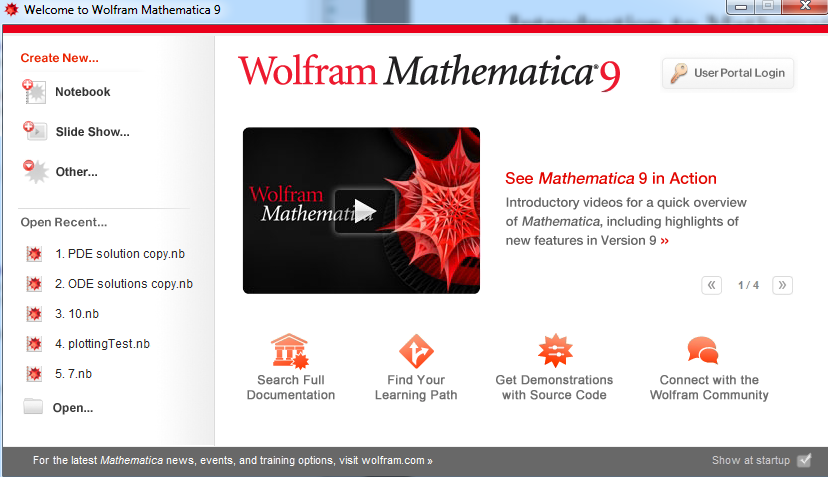
\includegraphics[scale=0.4]{figures/mathematica}
  \caption{Initialization interface of Mathematica}
  \label{fig:mathematica}
\end{figure}

\section{Tutorial}
There are many online tutorials that could help you learning \emph{Wolfram Language} and \emph{Mathematica}. You could find detailed tutorial at \href{http://reference.wolfram.com/language/?source=nav}{\color{blue} Wolfram Language \string& System Documentation Center}\footnote{\url{http://reference.wolfram.com/language/?source=nav}}. Those topics include:
\begin{itemize}
\item Core Language \string& Structure
\item Symbolic \string& Numeric Computation
\item Data Manipulation \string& Analysis
\item Visualization \string& Graphics
\item Images
\item ...
\end{itemize}

There are also many free video courses for educators and researchers which can be found at \href{http://www.wolfram.com/training/courses/edu001.html}{\color{blue} Mathematica for Teaching and Education.}\footnote{\url{http://www.wolfram.com/training/courses/edu001.html}} and
\href{http://www.wolfram.com/training/courses/edu002.html}{\color{blue} Mathematica for University Research}\footnote{\url{http://www.wolfram.com/training/courses/edu002.html}}. In the following section, we will look through some basics of \emph{Wolfram Language}.

\section{Basics}
\subsection{Simple Calculations}
In this section, we will see some examples on some basic arithmetic operations. The Wolfram Language is case sensitive. So
we should use \textbf{Sin} rather than \textbf{sin} to represent
a sinusoidal function.
\\~\\
\textbf{n = 3 + 6}\\
$9$
\\~\\
\textbf{n = 2 + 7 - 8/6}\\
$\frac{23}{3}$
\\~\\
\textbf{Sin[Pi/6]}\\
$\frac{1}{2}$
\\~\\
\textbf{n = Sin[30 Degree]}\\
$\frac{1}{2}$
\\~\\
\textbf{N [Sin[Pi/6]]}\\
$0.5$

\subsection{Matrix Operations}
Vectors and matrices in the Wolfram Language are simply represented by lists and by lists of lists, respectively.
Some basic matrix operations are as shown in Table~\ref{table:matrixOps}.
~\\\\
Expressions of a $3\times3$ matrix:\\
\textbf{m=\{\{-9,19,3\},\{-3,7,1\},\{-7,17,2\}\}}\\
\{\{-9, 19, 3\}, \{-3, 7, 1\}, \{-7, 17, 2\}\}

~\\
Transposing matrix \textbf{m}:\\
\textbf{Transpose[m]}\\
\{\{-9, -3, -7\}, \{19, 7, 17\}, \{3, 1, 2\}\}

~\\
Expressing \textbf{m} in matrix form\textbf{m}:\\
\textbf{MatrixForm[m]}\\
$\left(
\begin{array}{ccc}
 -9 & 19 & 4 \\
 -3 & 7 & 1 \\
 -7 & 17 & 2 \\
\end{array}
\right)$
\\~\\
Inversing matrix \textbf{m}:\\
\textbf{Inverse[m]}\\
$
\left(
\begin{array}{ccc}
 -\frac{3}{2} & \frac{13}{2} & -1 \\
 -\frac{1}{2} & \frac{3}{2} & 0 \\
 -1 & 10 & -3 \\
\end{array}
\right)
$

\begin{table}[H]
\caption{Basic matrix operations} % title of Table
\centering % used for centering table
\begin{tabular}{c c}
\hline %inserts double horizontal lines
Function & Purpose\\
%heading
\hline % inserts single horizontal line
Transpose[m] & Transpose $m^T$ \\
ConjugateTranspose[m] & Conjugate transpose $m^*$ (Hermitian conjugate) \\
Inverse[m] & Matrix inverse\\
Det[m] & Determinant\\
Tr[m] & Trace\\
MatrixRank[m] & Rank of matrix\\
[1ex] % [1ex] adds vertical space
\hline %inserts single line
\end{tabular}
\label{table:matrixOps} % is used to refer this table in the text
\end{table}

\subsection{Plotting}
The Wolfram Language has many ways to plot functions and data by using function \textbf{Plot}. And it has many options on what the scales should be, how the axes should be draw and so on. In this section, we will see some basic examples on data plotting.
\textbf{Plot[Sin[x], {x, 0, 10}]} gives result shown in Figure \ref{fig:sin}. \textbf{Plot3D[Sin[x]Cos[y], \{x, 0, 5\}, \{y, 1, 10\}]} produces result shown in Figure \ref{fig:sin3D}.\\
\textbf{Plot[Sin[x\string^2],\{x,0,3\},AxesLabel->\{"x value",Sin[x\string^2]\},GridLines->Automatic]} adds label and grid line to the plotting shown in Figure \ref{fig:sinLabel}.
%2\string^3 gives 2^3

\begin{figure}[H]
  \centering
    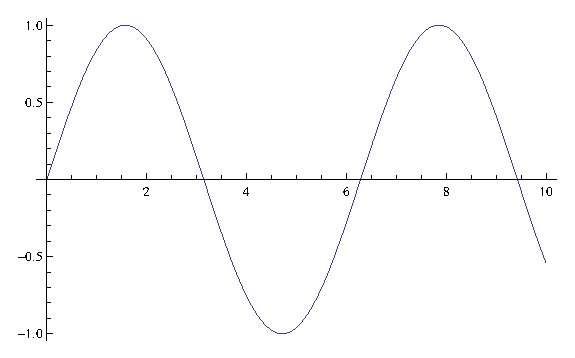
\includegraphics[scale=1]{figures/sin}
  \caption{Plot of $y=sin(x)$}
  \label{fig:sin}
\end{figure}

\begin{figure}[H]
  \centering
    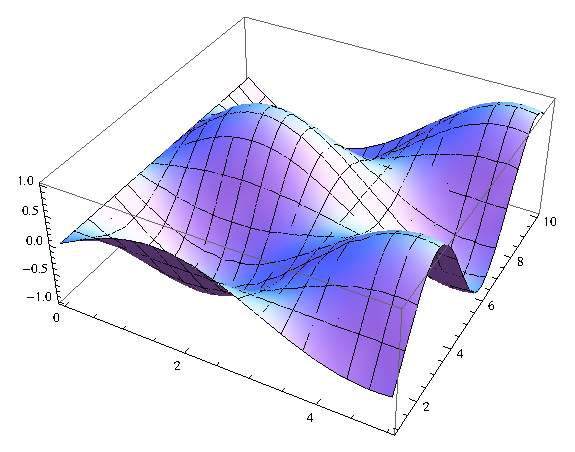
\includegraphics[scale=0.75]{figures/sin3D}
  \caption{Plot of $z=sin(x)cos(y)$}
  \label{fig:sin3D}
\end{figure}

\begin{figure}[H]
  \centering
    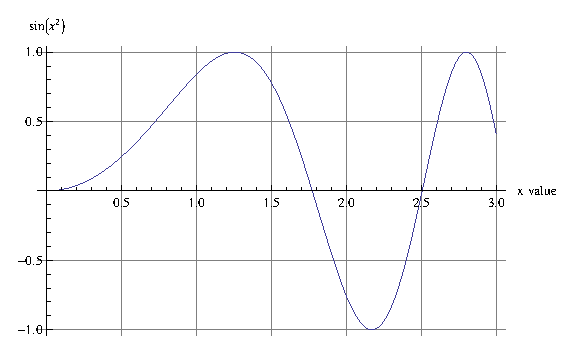
\includegraphics[scale=1]{figures/sinLabel}
  \caption{Plot of $y=sin(x^2)$ with label and axis description}
  \label{fig:sinLabel}
\end{figure}

\subsection{Solving Differential Equation}
Differential equations have three basic types of equations including:
\begin{itemize}
\item \emph{Ordinary Differential Equations} (ODEs), in which there is a single independent variable \textit{t} and one or more dependent variables $x_i(t)$.
\item \emph{Partial Differential Equations} (PDEs), in which there are two or more independent variables and one dependent variable.
\item \emph{Differential-Algebraic Equations} {DAEs}, in which some members of the system are differential equations and the others are purely algebraic, having no derivatives in them.
\end{itemize}

The function \emph{DSolve} gives symbolic solutions to the differential equations while function \emph{NDSolve} generates a general numerical differential equation solver. \emph{DSolve} is powerful in solving ODEs and most first-order PDEs as well as a limited number of the second-order PDEs. For DAEs, it is difficult to find the exact solutions, but \emph{DSolve} can solve many examples of such systems that occur in application.

\subsubsection{Example of solving ODE:}

\begin{figure}[hb]
  \centering
    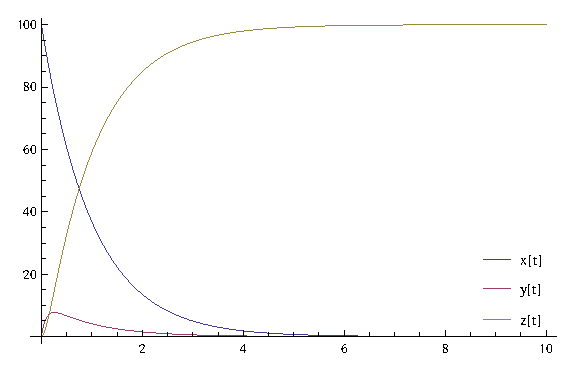
\includegraphics[scale=1]{figures/ODE}
  \caption{Plot of ODE solution}
  \label{fig:ODE}
\end{figure}

\definecolor{light-gray}{gray}{0.95}

%setting
\lstset{
language=Mathematica,
basicstyle=\small\sffamily,
%numbers=left,
%numberstyle=\tiny,
frame=tb,
columns=fullflexible,
showstringspaces=false,
mathescape=true,
escapechar=\@
%backgroundcolor=\color{light-gray}
}

%insert mathematica code
\begin{lstlisting}[caption=ODE solution,
  label=code:ode]
eqns = Join[
{x'[t]== -x[t], y'[t]== x[t] - 10y[t], 
z'[t]== 10y[t],
x[0]==100,y[0]==0, z[0]==0},
{x,y,z}, {t,100}];
sol = NDSolve[eqns];
Plot[
Evaluate[{x[t],y[t],z[t]} /. sol], 
{t,0,10}, 
PlotLegends->Placed[{"x[t]", "y[t]", "z[t]"} , {Right, Bottom}]]
\end{lstlisting}

In this example, we will solve the following ODEs.\\
\begin{equation*}
\left\{
\begin{aligned}
x'[t]&= -x[t],\\
y'[t]&= x[t] - 10y[t],\\
z'[t]&= y[t]
\end{aligned}
\right.
\end{equation*}
where initial conditions are x[0]=100, y[0]=0, z[0]=0 and $t\in[0,100]$.
First, we would use function Join[$list_1, list_2$, ...] to concatenates lists of equations and 
initial conditions into a new list. Then, we use function NDSolve[\textit{eqns}, $u$, {x, $x_{min}$, $x_{max}$}] to compute the numerical solution from the list gotten from Join. Finally, we use function Plot[{$f_1$, $f_2$, ...}, {$x$, $x_{min}$, $x_{max}$}] to draw all the curves of x[t], y[t] and z[t]. The code is as shown in Listing \ref{code:ode} and the curves are shown as Figure \ref{fig:ODE}. For detailed usages of function Join, NDSolve and Plot, please refer to the on-line \emph{Mathematica reference}.





\bibliographystyle{plain}
\bibliography{bibliography/MathematicaTutorial}
\end{document}